\section{Photoproduction with linearly polarized beam}%
\label{sec:photoprod}

\subsection{Moment decomposition}%
\label{sec:photoprod:moment}

Systems of two distinguishable spinless particles can also be produced
in photo-production reactions using stationary proton targets.  As in
the case of diffractive reactions discussed in \cref{sec:diffraction},
we are interested in the intermediate meson resonances~$X$ that are
produced in these reactions and that decay into the observed
two-(pseudo)scalar system.  A typical example for such a process is
the reaction
\begin{equation}
  \gamma\, p \to X^0\, p \to \etaOrPr\pi^0\, p,
\end{equation}
which is shown in \cref{fig:photoprod_etaprimepi}.  How to analyze
these reactions was studied in detail by the JPAC collaboration
in~\refsCite{Mathieu:2019fts,Mathieu:2019gxo}.  We will follow these
references here and will derive some equations.

\begin{figure}[tbp]
  \centering%
  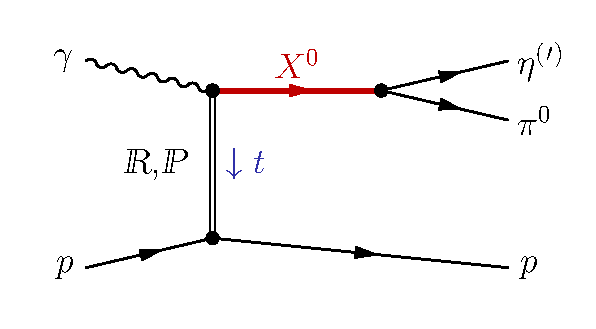
\includegraphics[width=0.5\textwidth]{photoproduction_x_etaprimepi_p}%
  \caption{Scattering of a real photon off a target proton mediated by
  Reggeon exchange.  In this photoproduction process, an intermediate
  state~$X^0$ with well-defined quantum numbers is produced, which in
  the example given here decays into the \etaOrPrPim channel.
  (\Confer~\cref{fig:diffractive_etaprimepi}.)}%
  \label{fig:photoprod_etaprimepi}%
\end{figure}

The analysis is based on the measured intensity distribution, \ie the
number density of events, which is decomposed into partial-wave
amplitudes analogous to the diffractive case in
\cref{eq:diffraction_intensity}:\footnote{\label{fn:photoprod_ampl_redef}This
corresponds to Eq.~(A3) in \refCite{Mathieu:2019fts} with the
phase-space factor~$\kappa$ absorbed into the partial-wave amplitudes,
\ie with the redefinition $\mathcal{T} \to \mathcal{T} /
\sqrt{\kappa}$ (see also footnote~6 in \refCite{Mathieu:2019fts}), and
with Eq.~(A5) inserted.}\todo{Can we express this as
$\abs{\text{amplitude}}^2$?}
\begin{equation}
  \label{eq:photoprod_intensity}
  \mathcal{I}(\Omega, \Phi; w, t)
  = \frac{\dif{N}}{\dif{w}\, \dif{t}\, \dif{\Omega}\, \dif{\Phi}}
  = \sum_{\substack{\ell m \\ \ell' m'}}^\infty
  Y_\ell^m(\Omega)~
  \dUnderbrace{\sum_{\substack{\lambda = \pm 1 \\ \mathclap{\lambda_1, \lambda_2 = \pm 1/2}}}
  \mathcal{T}^\ell_{\!m\, \lambda; \lambda_1\, \lambda_2}(w, t)\,
  \varrho^\gamma_{\lambda\, \lambda'}(\Phi)\,
  \mathcal{T}^{\ell' *}_{\!m'\, \lambda'; \lambda_1\, \lambda_2}(w, t)}{\equiv \varrho^{\ell\, \ell'}_{m\, m'}(w, t, \Phi)}~
  Y_{\ell'}^{m' *}(\Omega).
\end{equation}
Here, $N$~is the (acceptance-corrected) number of measured events,
$w$~is the invariant mass of the two-(pseudo)scalar system, $t$~is the
squared four-momentum transferred from the beam to the target
particle, $\Omega = (\theta, \phi)$ is the direction of one of the two
(pseudo)scalar mesons the~$X$ decays into, measured in the
Gottfried-Jackson or helicity rest frame of~$X$, and $\Phi$ is the
azimuthal\todo{Correct?} angle between the polarization vector of the
linearly polarized photon and the reaction plane in the $X$~rest
frame.  The $\mathcal{T}^\ell_{\!m\, \lambda; \lambda_1\,
\lambda_2}(w, t)$ are the partial-wave amplitudes that correspond to
an intermediate state with a spin, which is given by the relative
orbital angular momentum~$\ell$ between the two-(pseudo)scalar mesons,
and a spin projection~$m$ \wrt the chosen quantization axis
(Gottfried-Jackson frame: beam direction; helicity frame: momentum
direction of~$X$).  This intermediate state is produced in the
interaction of a photon with helicity~$\lambda = \pm 1$ and a target
proton with helicity~$\lambda_1 = \pm 1/2$; the recoil proton has
helicity~$\lambda_2 = \pm 1/2$.  The angular distribution of the
$X$~decay products is given by the spherical harmonics
$Y_\ell^m(\Omega)$~\cite{wikipedia:sphericalHarm}; the dependence on
the polarization angle~$\Phi$ by the photon spin-density
matrix~$\mat{\upvarrho}^\gamma(\Phi)$.  In
\cref{eq:photoprod_intensity}, $\varrho^{\ell\, \ell'}_{m\, m'}(w, t,
\Phi)$ is the spin-density matrix element of~$X$ analogous to the
diffractive case in \cref{eq:diffraction_intensity_refl_spin-dens}.

Using the fact that the three Pauli matrices $\vec{\mat{\upsigma}} =
(\mat{\upsigma}_1, \mat{\upsigma}_2, \mat{\upsigma}_3)^T$ and
$\mat{I}_{2 \times 2}$ form a complete set in the space of Hermitian
$2 \times 2$ matrices, we can expand $\mat{\upvarrho}^\gamma(\Phi)$,
\ie
\begin{equation}
  \mat{\upvarrho}^\gamma(\Phi)
  = \frac{1}{2}\, \mat{I}_{2 \times 2} + \frac{1}{2}\, \vec{P}_\gamma(\Phi) \cdot \vec{\mat{\upsigma}}.
\end{equation}
Here, $\vec{P}_\gamma(\Phi)$ describes the photon polarization.  Its
length~$0 \leq P_\gamma \leq 1$ is the degree of polarization and its
direction depends on the kind of polarization:\footnote{See Eq.~(19)
in \refCite{Schilling:1969um}.}
\begin{equation}
  \vec{P}_\gamma(\Phi)
  = \begin{cases*}
    P_\gamma\, (0, 0, \lambda)^T                & for circularly polarized photons with $\lambda = \pm 1$, \\
    -P_\gamma\, (\cos 2 \Phi, \sin 2 \Phi, 0)^T & for linearly polarized photons with polarization angle~$\Phi$.
  \end{cases*}
\end{equation}
Hence, for linearly polarized photons, the intensity distribution in
\cref{eq:photoprod_intensity} can be written as the sum of three
terms:\footnote{See Eq.~(B4) in \refCite{Mathieu:2019fts}.}
\begin{equation}
  \label{eq:photoprod_intensity_sum}
  \mathcal{I}(\Omega, \Phi; w, t)
  = \mathcal{I}_0(\Omega; w, t)
  - \mathcal{I}_1(\Omega; w, t)\, P_\gamma\, \cos 2 \Phi
  - \mathcal{I}_2(\Omega; w, t)\, P_\gamma\, \sin 2 \Phi
\end{equation}
with the intensity components
\begin{equation}
  \label{eq:photoprod_intensity_components}
  \mathcal{I}_i(\Omega; w, t)
  = \sum_{\substack{\ell m \\ \ell' m'}}^\infty
  Y_\ell^m(\Omega)\,
  \prescript{i}{}{\varrho}^{\ell\, \ell'}_{m\, m'}(w, t)\,
  Y_{\ell'}^{m' *}(\Omega);
  \quad i = 0, 1, 2
\end{equation}
and the spin-density matrix components\footnote{See Eq.~(11) in
\refCite{Mathieu:2019fts}.}
\begin{align}
  \label{eq:photoprod_rho_0}
  \prescript{0}{}{\varrho}^{\ell\, \ell'}_{m\, m'}(w, t)
  ={}& \frac{1}{2}\quad \sum_{\substack{\lambda = \pm 1 \\ \mathclap{\lambda_1, \lambda_2 = \pm 1/2}}}
  \mathcal{T}^\ell_{\!m\, \lambda; \lambda_1\, \lambda_2}(w, t)\,
  \mathcal{T}^{\ell' *}_{\!m'\, \lambda; \lambda_1\, \lambda_2}(w, t)
  \\
  \label{eq:photoprod_rho_1}
  \prescript{1}{}{\varrho}^{\ell\, \ell'}_{m\, m'}(w, t)
  ={}& \frac{1}{2}\quad \sum_{\substack{\lambda = \pm 1 \\ \mathclap{\lambda_1, \lambda_2 = \pm 1/2}}}
  \mathcal{T}^\ell_{\!m\, {-\lambda}; \lambda_1\, \lambda_2}(w, t)\,
  \mathcal{T}^{\ell' *}_{\!m'\, \lambda; \lambda_1\, \lambda_2}(w, t)
  \\
  \label{eq:photoprod_rho_2}
  \prescript{2}{}{\varrho}^{\ell\, \ell'}_{m\, m'}(w, t)
  ={}& \frac{\imag}{2}\quad \sum_{\substack{\lambda = \pm 1 \\ \mathclap{\lambda_1, \lambda_2 = \pm 1/2}}}
  \lambda\,
  \mathcal{T}^\ell_{\!m\, {-\lambda}; \lambda_1\, \lambda_2}(w, t)\,
  \mathcal{T}^{\ell' *}_{\!m'\, \lambda; \lambda_1\, \lambda_2}(w, t).
\end{align}
Note that neither the $\mathcal{I}_i$ nor the
$\prescript{i}{}{\varrho}^{\ell\, \ell'}_{m\, m'}$ depend on~$\Phi$.
Furthermore, the spin-density matrix elements of~$X$ in
\cref{eq:photoprod_intensity} are given by
\begin{equation}
  \label{eq:photoprod_spin_dens_sum}
  \varrho^{\ell\, \ell'}_{m\, m'}(w, t, \Phi)
  = \prescript{0}{}{\varrho}^{\ell\, \ell'}_{m\, m'}(w, t)
  - \prescript{1}{}{\varrho}^{\ell\, \ell'}_{m\, m'}(w, t)\, P_\gamma\, \cos 2 \Phi
  - \prescript{2}{}{\varrho}^{\ell\, \ell'}_{m\, m'}(w, t)\, P_\gamma\, \sin 2 \Phi.
\end{equation}

In \cref{eq:photoprod_intensity_sum}, the three intensity components
$\mathcal{I}_i(\Omega; w, t)$ (as well as the three spin-density
matrix components in \cref{eq:photoprod_spin_dens_sum}) are modulated
by different $\Phi$~dependences.  $\mathcal{I}_0(\Omega; w, t)$ is the
unpolarized intensity and hence constant in~$\Phi$.  It is equivalent
to the intensity for the diffractive case in
\cref{eq:diffraction_intensity_refl_spin-dens}.  The other two
components $\mathcal{I}_{1, 2}(\Omega; w, t)$ depend on the photon
polarization and are hence modulated by different $\Phi$~dependences.
Note that the functions $\cBrk[1]{f_0(\Phi), f_1(\Phi), f_2(\Phi)} =
\cBrk[1]{1, \cos 2 \Phi, \sin 2 \Phi}$ that modulate the intensity
components constitute an orthogonal set of functions, \ie
\begin{equation}
  \label{eq:photoprod_orthogonality_phi}
  \int_{-\pi}^{+\pi}\!\!\! \dif{\Phi}\, f_i(\Phi)\, f_j(\Phi)
  = (1 + \delta_{i 0}) \pi\, \delta_{i j};
  \quad i, j = 0 ,1, 2.
\end{equation}

Like for the diffractive case, the partial-wave analysis as well as
the moment decomposition are performed in narrow kinematic cells in
the $(w, t)$ plane, assuming that within each cell all quantities are
in good approximation independent of~$w$ and~$t$.  To simplify
notation we hence omit the~$w$ and $t$~dependencies in all formulas
below, \ie these formulas are valid in a given $(w, t)$ cell.

We decompose the intensity in \cref{eq:photoprod_intensity_sum} into
spherical harmonics to obtain the moments, analogously to the
diffractive case in \cref{eq:diffraction_intensity_moments}.  Due to
the orthogonality of the $\mathcal{I}_i$ terms in $\Phi$~space, we can
decompose each intensity component separately:\footnote{See Eq.~(A8)
in \refCite{Mathieu:2019fts}.}
\begin{align}
  \label{eq:photoprod_intensity_moments_norm_unpol}
  \mathcal{I}_0(\Omega)
  ={}& \sum_{L M}^\infty \sqrt{\frac{2 L + 1}{4 \pi}}\, H_0(L, M)\, Y_L^M(\Omega)
  \\
  \label{eq:photoprod_intensity_moments_norm_pol}
  \mathcal{I}_{1, 2}(\Omega)
  ={}& -\sum_{L M}^\infty \sqrt{\frac{2 L + 1}{4 \pi}}\, H_{1, 2}(L, M)\, Y_L^M(\Omega).
\end{align}
Here, we have used the same normalization as in
\cref{sec:diffraction:moments_norm}.
\Cref{eq:photoprod_intensity_moments_norm_unpol} is equivalent to
\cref{eq:diffraction_intensity_moments_norm}.  The minus sign in
\cref{eq:photoprod_intensity_moments_norm_pol} is introduced in order
to compensate that the corresponding intensity components contribute
negatively to the intensity distribution in
\cref{eq:photoprod_intensity_sum}.\footnote{Equivalently, the minus
sign ensures that $H_1(0, 0) \geq 0$ for positive-reflectivity waves
(see \cref{sec:photoprod:reflectivity} and Appendix~D in
\refCite{Mathieu:2019fts}).\todoInl{pick this up again in
\cref{sec:photoprod:reflectivity}}}

The corresponding moments are
\begin{align}
  \label{eq:photoprod_moments_norm_unpol}
  H_0(L, M)
  ={}& \frac{1}{2 \pi}\, \sqrt{\frac{4 \pi}{2 L + 1}}\, \int_{4 \pi}\!\!\! \dif{\Omega}\, \int_{-\pi}^{+\pi}\!\!\! \dif{\Phi}\,
  \mathcal{I}(\Omega, \Phi)\, Y_L^{M *}(\Omega)
  \\
  \label{eq:photoprod_moments_norm_pol}
  H_{1, 2}(L, M)
  ={}& \frac{1}{P_\gamma}\, \frac{1}{\pi}\, \sqrt{\frac{4 \pi}{2 L + 1}}\, \int_{4 \pi}\!\!\! \dif{\Omega}\, \int_{-\pi}^{+\pi}\!\!\! \dif{\Phi}\,
  \mathcal{I}(\Omega, \Phi)\, Y_L^{M *}(\Omega) \times \begin{cases*}
    \cos 2 \Phi & for $i = 1$, \\
    \sin 2 \Phi & for $i = 2$.
  \end{cases*}
\end{align}
Here, $H_0(L, M)$ becomes identical to
\cref{eq:diffraction_moments_norm} for the diffractive case if the
intensity distribution is independent of~$\Phi$.  The two polarized
moments $H_{1, 2}(L, M)$ represent orthogonal angular distributions
in~$\Phi$ (see \cref{eq:photoprod_orthogonality_phi}).


\subsection{Relation between moments and partial-wave amplitudes}%
\label{sec:photoprod:moments_pw}

As in the diffractive case, we see that the moments are linear
combinations of the corresponding components of the spin-density
matrix of~$X$ by inserting \cref{eq:spherical_harm_prod} into
\cref{eq:photoprod_intensity_components} and comparing with
\cref{eq:photoprod_intensity_moments_norm_unpol,eq:photoprod_intensity_moments_norm_pol},
\ie\footnote{See Eq.~(A9) in \refCite{Mathieu:2019fts}.}
\begin{align}
  \label{eq:photoprod_moment_unpol_pw}
  H_0(L, M)
  ={}& \sum_{\substack{\ell m \\ \ell' m'}}^\infty \sqrt{\frac{2 \ell' + 1}{2 \ell + 1}}
  \clebsch{\ell'}{0}{L}{0}{\ell}{0}\, \clebsch{\ell'}{m'}{L}{M}{\ell}{m}\,
  \prescript{0}{}{\varrho}^{\ell\, \ell'}_{m\, m'}
  \\
  \label{eq:photoprod_moment_pol_pw}
  H_{1, 2}(L, M)
  ={}& -\sum_{\substack{\ell m \\ \ell' m'}}^\infty \sqrt{\frac{2 \ell' + 1}{2 \ell + 1}}
  \clebsch{\ell'}{0}{L}{0}{\ell}{0}\, \clebsch{\ell'}{m'}{L}{M}{\ell}{m}\,
  \prescript{1, 2}{}{\varrho}^{\ell\, \ell'}_{m\, m'},
\end{align}
where the $\prescript{i}{}{\varrho}^{\ell\, \ell'}_{m\, m'}$ are given
by \crefrange{eq:photoprod_rho_0}{eq:photoprod_rho_2}.  For given~$(L,
M)$, the Clebsch-Gordan coefficients restrict the sums to those
quantum-number combinations, for which $\ell' + L + \ell =
\text{even}$ (see \cref{eq:ang_mom_sum}), $\abs{\ell' - L} \leq \ell
\leq \ell' + L$, and $m = m' + M$.  Conversely, this means that a
partial-wave amplitude with orbital angular momentum~$\ell$
contributes to all moments~$H_i$ with~$L$ from~0 up to $2 \ell$.


\subsection{Symmetry properties of moments}%
\label{sec:photo_prod:moments_sym}

We use the same arguments as in \cref{sec:diffraction:moments_sym} to
derive the symmetry relations for the photoproduction moments.

Using the definition of the moments in
\cref{eq:photoprod_moments_norm_unpol,eq:photoprod_moments_norm_pol}
together with the symmetry property of the spherical harmonics in
\cref{eq:spherical_harm_sym}, we see that
\begin{align}
  H_0^*(L, M)
  ={}& (-1)^M\, \frac{1}{2 \pi}\, \sqrt{\frac{4 \pi}{2 L + 1}}\, \int_{4 \pi}\!\!\! \dif{\Omega}\, \int_{-\pi}^{+\pi}\!\!\! \dif{\Phi}\,
  \mathcal{I}(\Omega, \Phi)\, Y_L^{(-M) *}(\Omega) \notag
  \\
  \label{eq:photoprod_moment_unpol_sym_1}
  ={}& (-1)^M\, H_0(L, {-M})
  \\
  \label{eq:photoprod_moment_pol_sym_1}
  H_{1, 2}^*(L, M)
  ={}& (-1)^M\, \frac{1}{P_\gamma}\, \frac{1}{\pi}\, \sqrt{\frac{4 \pi}{2 L + 1}}\, \int_{4 \pi}\!\!\! \dif{\Omega}\, \int_{-\pi}^{+\pi}\!\!\! \dif{\Phi}\,
  \mathcal{I}(\Omega, \Phi)\, Y_L^{(-M) *}(\Omega) \times \begin{cases*}
    \cos 2 \Phi & for $i = 1$, \\
    \sin 2 \Phi & for $i = 2$
  \end{cases*}
  \notag
  \\
  ={}& (-1)^M\, H_{1,2}(L, {-M}),
\end{align}
which is analogous to \cref{eq:diffraction_moment_sym_1}.

Since the formulas for the intensity components in
\cref{eq:photoprod_intensity_moments_norm_unpol,eq:photoprod_intensity_moments_norm_pol}
have---up to overall signs---the same form as
\cref{eq:diffraction_intensity_moments_norm}, we can use exactly the
same arguments as in \cref{eq:diffraction_intensity_moments_general}
to see that all intensity components are real-valued and that only the
moments with $M \geq 0$ are required, \ie
\begin{align}
  \label{eq:photoprod_intensity_moments_unpol_general}
  \mathcal{I}_0(\Omega)
  ={}& \sum_{L = 0}^\infty \sqrt{\frac{2 L + 1}{4 \pi}} \sum_{M = 0}^{L} (2 - \delta_{M 0})\, \Re{H_0(L, M)\, Y_L^M(\Omega)}
  \\
  \label{eq:photoprod_intensity_moments_pol_general}
  \mathcal{I}_{1, 2}(\Omega)
  ={}& -\sum_{L = 0}^\infty \sqrt{\frac{2 L + 1}{4 \pi}} \sum_{M = 0}^{L} (2 - \delta_{M 0})\, \Re{H_{1, 2}(L, M)\, Y_L^M(\Omega)}.
\end{align}

We use the relation of the moments to the partial-wave amplitudes in
\cref{eq:photoprod_moment_unpol_pw,eq:photoprod_moment_pol_pw}
together with the symmetry properties of the Clebsch-Gordan
coefficients in \cref{eq:clebsch_sym} to show that
\begin{align}
  H(L, -M)
  = \sum_{\substack{\ell m \\ \ell' m'}}^\infty \sqrt{\frac{2 \ell' + 1}{2 \ell + 1}}
  \clebsch{\ell'}{0}{L}{0}{\ell}{0}\, (-1)^{L - M}\, \clebsch{\ell}{m}{L}{M}{\ell'}{m'}\,
  \prescript{0}{}{\varrho}^{\ell\, \ell'}_{m\, m'}
  = (-1)^{L - M}\,  H(L, M)
\end{align}


\subsection{Reflectivity basis}%
\label{sec:photoprod:reflectivity}

In Appendix~D of \refCite{Mathieu:2019fts}, the reflectivity basis is
introduced by defining the partial-wave amplitudes in the reflectivity
basis\footnote{See Eq.~(D1) in
\refCite{Mathieu:2019fts}.}\footnote{Alternative approaches to apply
the reflectivity basis are discussed in \refCite{Salgado:2020}.}
\begin{equation}
  \label{eq:photoprod_amplitude_refl}
  \prescript{\refl}{}{\mathcal{T}}^\ell_{\!m; \lambda_1\, \lambda_2}
  \equiv \frac{1}{2}\, \sBrk{\mathcal{T}^\ell_{\!m\, {+1}; \lambda_1\, \lambda_2}
  - \refl\, (-1)^m\, \mathcal{T}^\ell_{\!{-m}\, {-1}; \lambda_1\, \lambda_2}},
\end{equation}
which are linear combinations of the partial-wave amplitudes with
opposite photon helicities~$\lambda$ and opposite $X$~spin projection
quantum numbers~$m$, where $m = -\ell, \ldots, +\ell$.  Hence, the
reflectivity quantum number $\refl = \pm$ effectively replaces the
photon helicity $\lambda = \pm 1$ such that the total number of
amplitudes for given~$\ell$ and~$m$ remains unchanged.

Formulating the intensity model in the reflectivity basis has the
advantage that in the high-energy limit at leading order~\refl
corresponds to the naturality of the spin-parity exchanged in the
scattering process (see Appendices~C and~D in
\refCite{Mathieu:2019fts}).  Another advantage of the reflectivity
basis is that due to parity conservation partial-wave amplitudes with
opposite~\refl do not interfere.\footnote{See Eq.~(D5) in
\refCite{Mathieu:2019fts}.}  Parity also directly relates partial-wave
amplitudes with opposite helicities of the target and the recoil
proton, \ie\footnote{See Eq.~(D3) in \refCite{Mathieu:2019fts}.}
\begin{equation}
  \prescript{\refl}{}{\mathcal{T}}^\ell_{\!m; {-\lambda_1}\, {-\lambda_2}}
  = \refl\, (-1)^{\lambda_1 - \lambda_2}\, \prescript{\refl}{}{\mathcal{T}}^\ell_{\!m; \lambda_1\, \lambda_2}.
\end{equation}
Therefore, for given~\refl, $\ell$, and~$m$, only two of the four
possible partial-wave amplitudes are independent,\footnote{In general,
for scattering reactions with a recoil particle with spin~$J_R$, there
will be $2 J_R + 1$ independent amplitudes $\sBrk{\ell}^{(\refl)}_{m;
k}$ with $k = 0, \ldots, 2 J_R$.} namely the proton spin-flip
amplitude\footnote{See Eq.~(D4) in \refCite{Mathieu:2019fts}.}
\begin{align}
  \prescript{\refl}{}{\mathcal{T}}^\ell_{\!m; {+1}\, {-1}}
  \equiv{}& \sBrk{\ell}^{(\refl)}_{m; 0}
  \intertext{and the proton spin-non-flip amplitude}
  \prescript{\refl}{}{\mathcal{T}}^\ell_{\!m; {+1}\, {+1}}
  \equiv{}& \sBrk{\ell}^{(\refl)}_{m; 1}.
\end{align}
Furthermore, since parity is conserved the spin-flip and spin-non-flip
amplitudes do not interfere. In the conventional basis, incorporating
these parity constraints into
\crefrange{eq:photoprod_intensity_components}{eq:photoprod_rho_2} is
difficult because parity relates amplitudes that in addition to
opposite~$\lambda_1$ and~$\lambda_2$ quantum numbers also have
opposite~$m$ and~$\lambda$.\footnote{See Eq.~(A14) in
\refCite{Mathieu:2019fts}.}  However, in the reflectivity basis we can
simply write\footnote{See Eq.~(D7) in \refCite{Mathieu:2019fts}.}
\begin{equation}
  \label{eq:photoprod_rho_refl}
  \prescript{i}{}{\varrho}^{\ell\, \ell'}_{m\, m'}
  = \prescript{i}{}{\varrho}^{(+)\, \ell\, \ell'}_{m\, m'} + \prescript{i}{}{\varrho}^{(-)\, \ell\, \ell'}_{m\, m'};
  \quad i = 0, 1, 2
\end{equation}
with\footnote{See Eq.~(D8) in \refCite{Mathieu:2019fts} and
\cref{fn:photoprod_ampl_redef}.}
\begin{align}
  \label{eq:photoprod_rho_0_refl}
  \prescript{0}{}{\varrho}^{(\refl)\, \ell\, \ell'}_{m\, m'}
  ={}& \sum_{k = 0, 1} \rBrk[2]{\sBrk{\ell}^{(\refl)}_{m; k}\, \sBrk{\ell'}^{(\refl) *}_{m'; k}
  + (-1)^{m - m'}\, \sBrk{\ell}^{(\refl)}_{{-m}; k}\, \sBrk{\ell'}^{(\refl) *}_{{-m'}; k}}
  \\
  \label{eq:photoprod_rho_1_refl}
  \prescript{1}{}{\varrho}^{(\refl)\, \ell\, \ell'}_{m\, m'}
  ={}& -\refl \sum_{k = 0, 1} \rBrk[2]{(-1)^m\, \sBrk{\ell}^{(\refl)}_{{-m}; k}\, \sBrk{\ell'}^{(\refl) *}_{m'; k}
  + (-1)^{m'}\, \sBrk{\ell}^{(\refl)}_{m; k}\, \sBrk{\ell'}^{(\refl) *}_{{-m'}; k}}
  \\
  \label{eq:photoprod_rho_2_refl}
  \prescript{2}{}{\varrho}^{(\refl)\, \ell\, \ell'}_{m\, m'}
  ={}& -\imag\, \refl \sum_{k = 0, 1} \rBrk[2]{(-1)^m\, \sBrk{\ell}^{(\refl)}_{{-m}; k}\, \sBrk{\ell'}^{(\refl) *}_{m'; k}
  - (-1)^{m'}\, \sBrk{\ell}^{(\refl)}_{m; k}\, \sBrk{\ell'}^{(\refl) *}_{{-m'}; k}}.
\end{align}
In \cref{eq:photoprod_rho_refl}, we sum incoherently over~$\refl =
\pm$ and in
\crefrange{eq:photoprod_rho_0_refl}{eq:photoprod_rho_2_refl}, we sum
incoherently over~$k = 0, 1$, \ie the rank of the
$\prescript{i}{}{\varrho}^{(\refl)\, \ell\, \ell'}_{m\, m'}$ is in
general~2.

Note that usually neither the spin of the target proton nor the one of
the recoil proton is measured.  In this case, we cannot distinguish
experimentally between proton spin-flip and proton spin-non-flip
amplitudes.  Still, the intensity distribution obtained by inserting
\crefrange{eq:photoprod_rho_refl}{eq:photoprod_rho_2_refl} into
\cref{eq:photoprod_intensity_components} has two incoherent sectors
indexed by~$k = 0, 1$ as required by parity conservation, but $k$~has
no direct physical interpretation.  In practice, one often assumes
that either the spin-non-flip or the spin-flip amplitudes dominate and
sets $k = 0$.  This means the partial-wave amplitudes are all fully
coherent and the spin-density matrices in
\crefrange{eq:photoprod_rho_0_refl}{eq:photoprod_rho_2_refl} have
rank~1.


\subsection{!!!Relation between moments and partial-wave amplitudes}%

\todoInl{fix}
Inserting
\crefrange{eq:photoprod_rho_0_refl}{eq:photoprod_rho_2_refl}, we
obtain the relation between the moments and the partial-wave
amplitudes in the reflectivity basis defined in
\cref{sec:photoprod:reflectivity}:
\begin{align}
  \label{eq:photoprod_moment_0_pw_refl}
  H_0(L, M)
  ={}& \begin{multlined}[t][0.8\columnwidth]
    \sum_{\substack{\ell m \\ \ell' m'}}^\infty \sqrt{\frac{2 \ell' + 1}{2 \ell + 1}}
    \clebsch{\ell'}{0}{L}{0}{\ell}{0}\, \clebsch{\ell'}{m'}{L}{M}{\ell}{m} \\[-2ex]
    \shoveleft{\hfill \times%
      \sum_{\refl = \pm} \sum_{k = 0, 1} \rBrk[2]{\sBrk{\ell}^{(\refl)}_{m; k}\, \sBrk{\ell'}^{(\refl) *}_{m'; k}
      + (-1)^{m - m'}\, \sBrk{\ell}^{(\refl)}_{{-m}; k}\, \sBrk{\ell'}^{(\refl) *}_{{-m'}; k}}
    }
  \end{multlined}
  \\
  \label{eq:photoprod_moment_1_pw_refl}
  H_1(L, M)
  ={}& \begin{multlined}[t][0.8\columnwidth]
    \sum_{\substack{\ell m \\ \ell' m'}}^\infty \sqrt{\frac{2 \ell' + 1}{2 \ell + 1}}
    \clebsch{\ell'}{0}{L}{0}{\ell}{0}\, \clebsch{\ell'}{m'}{L}{M}{\ell}{m} \\[-2ex]
    \shoveleft{\hfill \times%
      \sum_{\refl = \pm} \refl \sum_{k = 0, 1} \rBrk[2]{(-1)^m\, \sBrk{\ell}^{(\refl)}_{{-m}; k}\, \sBrk{\ell'}^{(\refl) *}_{m'; k}
      + (-1)^{m'}\, \sBrk{\ell}^{(\refl)}_{m; k}\, \sBrk{\ell'}^{(\refl) *}_{{-m'}; k}}
    }
  \end{multlined}
  \\
  \label{eq:photoprod_moment_2_pw_refl}
  H_2(L, M)
  ={}& \begin{multlined}[t][0.8\columnwidth]
    \imag \sum_{\substack{\ell m \\ \ell' m'}}^\infty \sqrt{\frac{2 \ell' + 1}{2 \ell + 1}}
    \clebsch{\ell'}{0}{L}{0}{\ell}{0}\, \clebsch{\ell'}{m'}{L}{M}{\ell}{m} \\[-2ex]
    \shoveleft{\hfill \times%
      \sum_{\refl = \pm} \refl \sum_{k = 0, 1} \rBrk[2]{(-1)^m\, \sBrk{\ell}^{(\refl)}_{{-m}; k}\, \sBrk{\ell'}^{(\refl) *}_{m'; k}
      - (-1)^{m'}\, \sBrk{\ell}^{(\refl)}_{m; k}\, \sBrk{\ell'}^{(\refl) *}_{{-m'}; k}}
    }.
  \end{multlined}
\end{align}
It is important to note that each moment is an incoherent sum of
contributions from both reflectivities, \ie the moments do not
separate these contributions.  Also note that in
\cref{eq:photoprod_moment_0_pw_refl} the contributions from the two
reflectivities enter with the same sign, whereas in
\cref{eq:photoprod_moment_1_pw_refl,eq:photoprod_moment_2_pw_refl}
they enter with opposite sign.

\todoInl{add text}
\begin{align}
  H_0(0, 0)
  ={}& \sum_{\ell m}^\infty \prescript{0}{}{\varrho}^{\ell\, \ell}_{m\, m}
  = \sum_{\ell m}^\infty \sum_{\refl = \pm} \sum_{k = 0, 1}
  \rBrk[2]{\Abs[1]{\sBrk{\ell}^{(\refl)}_{m; k}}^2 + \Abs[1]{\sBrk{\ell}^{(\refl)}_{{-m}; k}}^2} \notag
  \\
  ={}& 2 \sum_{\ell m}^\infty \sum_{k = 0, 1}
  \rBrk[2]{\Abs[1]{\sBrk{\ell}^{(+)}_{m; k}}^2 + \Abs[1]{\sBrk{\ell}^{(-)}_{m; k}}^2}
  \\
  H_1(0, 0)
  ={}& -\sum_{\ell m}^\infty \prescript{1}{}{\varrho}^{\ell\, \ell}_{m\, m}
  = \sum_{\ell m}^\infty \sum_{\refl = \pm} \refl \sum_{k = 0, 1}
  (-1)^m \rBrk[2]{\sBrk{\ell}^{(\refl)}_{{-m}; k}\, \sBrk{\ell}^{(\refl) *}_{m; k}
  + \sBrk{\ell}^{(\refl)}_{m; k}\, \sBrk{\ell}^{(\refl) *}_{{-m}; k}} \notag
  \\
  ={}& 2 \sum_{\ell m}^\infty \sum_{k = 0, 1}
  (-1)^m \Re[2]{\sBrk{\ell}^{(+)}_{m; k}\, \sBrk{\ell}^{(+) *}_{{-m}; k} - \sBrk{\ell}^{(-)}_{m; k}\, \sBrk{\ell}^{(-) *}_{{-m}; k}}
  \\
  H_2(0, 0)
  ={}& -\sum_{\ell m}^\infty \prescript{2}{}{\varrho}^{\ell\, \ell}_{m\, m}
  = \imag \sum_{\ell m}^\infty \sum_{\refl = \pm} \refl \sum_{k = 0, 1}
  (-1)^m \rBrk[2]{\sBrk{\ell}^{(\refl)}_{{-m}; k}\, \sBrk{\ell}^{(\refl) *}_{m; k}
  - \sBrk{\ell}^{(\refl)}_{m; k}\, \sBrk{\ell}^{(\refl) *}_{{-m}; k}} \notag
  \\
  ={}& 2 \sum_{\ell m}^\infty \sum_{k = 0, 1}
  (-1)^m \Im[2]{\sBrk{\ell}^{(+)}_{m; k}\, \sBrk{\ell}^{(+) *}_{{-m}; k} - \sBrk{\ell}^{(-)}_{m; k}\, \sBrk{\ell}^{(-) *}_{{-m}; k}}
\end{align}
